\documentclass[12pt,a4paper]{article}
\usepackage[utf8]{inputenc}
\usepackage{graphicx}
\usepackage{tikz}
\usetikzlibrary{fit}
\usepackage{lmodern}
\usepackage{sectsty}


\sectionfont{\color{cyan}}

\begin{document}
   \begin{titlepage}
      {\fontfamily{lmss}\selectfont
      	\centering
      	
\includegraphics[width=0.30\textwidth]{logo.png}\par\vspace{1cm}
      	{\LARGE Capstone Project Demo 1 \par}
      	\vspace{0.25cm}
      	{\huge\bfseries \color{cyan}System Requirements and Design Document\par}
      	\vspace{1cm}
      	{\Large\textit{by} Brute Force\par}
         \vspace{0.25cm}
         \begin{tikzpicture}
            \node [inner sep=0pt,,outer sep=0pt,clip,rounded corners=0.5cm] (pict) at (0,0) {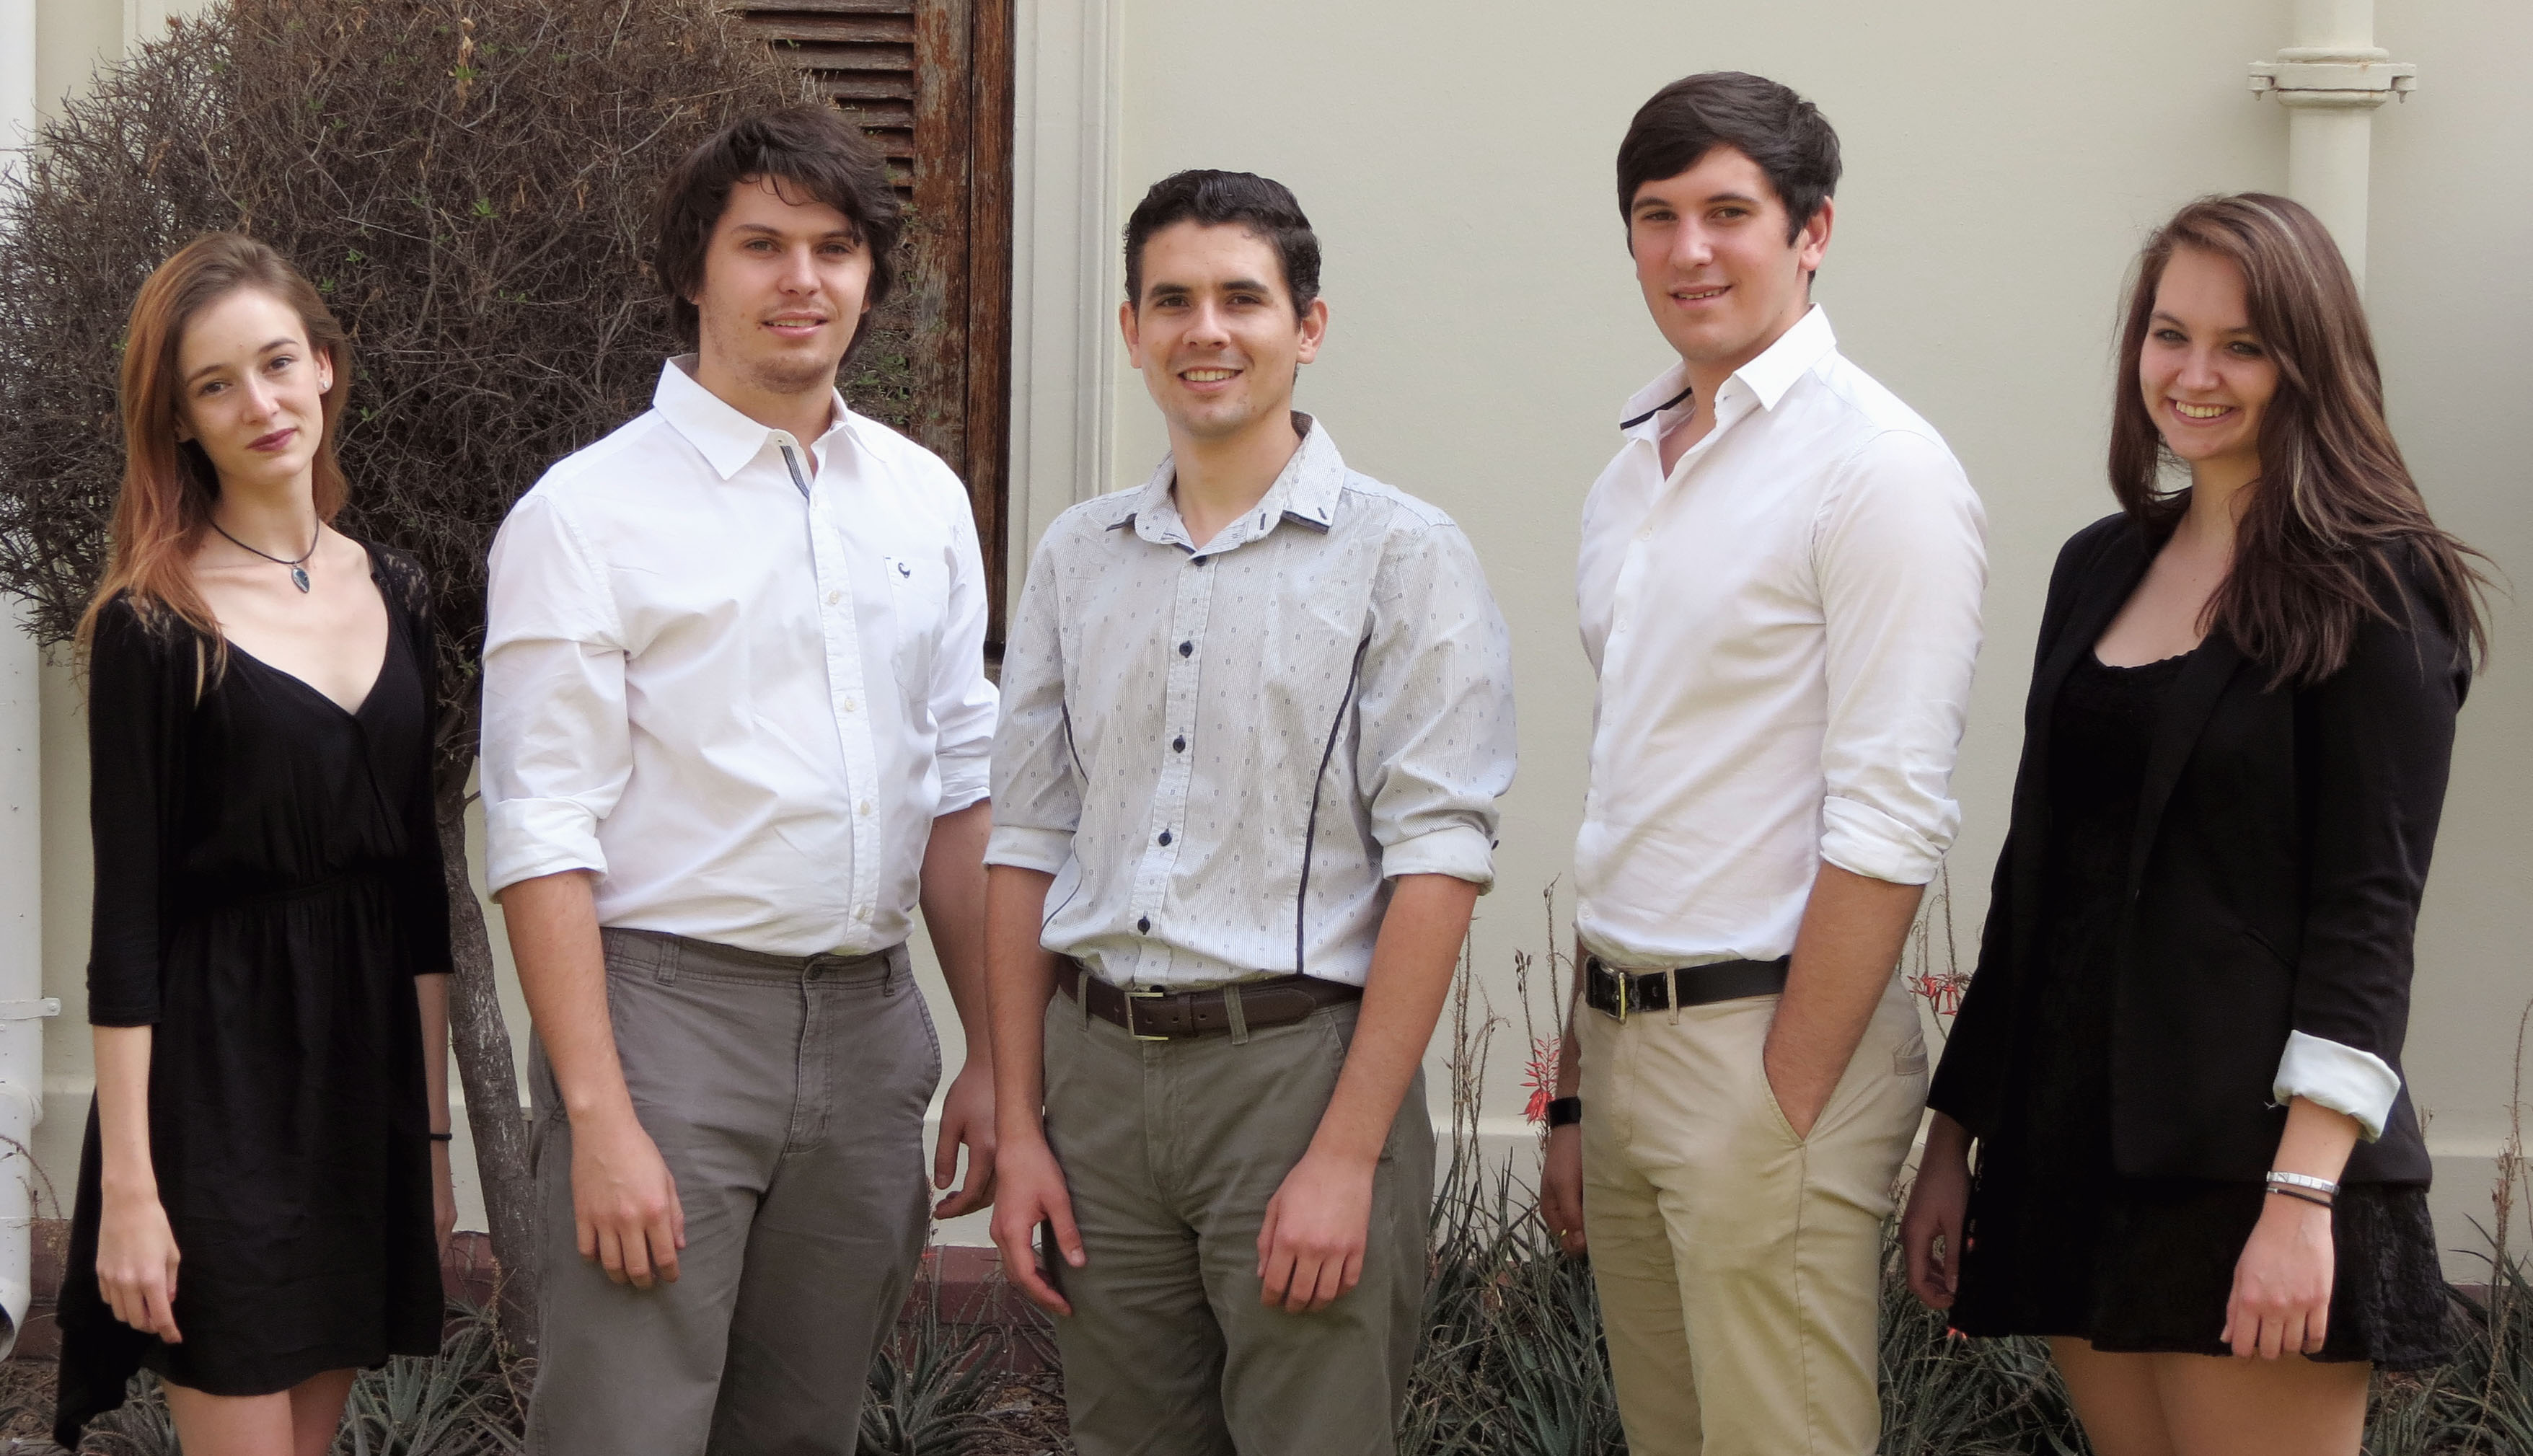
\includegraphics[width=0.9\textwidth]{team.jpg}};
            \node[fit=(pict),rounded corners=.55cm,inner sep=2pt]{};
         \end{tikzpicture}

         \par\vspace{1cm}
         \date{}
         \author{}
         \title{}
         \centering
         \textbf{Authors:}\\
         Mia Gerber\\
         Matthew Perry\\
         Wanrick Willemse\\
         Duart Breedt\\
         Linda Potgieter\\
      }
   \end{titlepage}
   \maketitle
   \tableofcontents
   \newpage

   \section{Introduction}
   	\subsection{Purpose}
   	
   	\subsection{Scope}
   		
   	\subsection{Overview}

   \section{Overall Description}
   	\subsection{System Interfaces}
   	
   	\subsection{User Interfaces}
   		
   	\subsection{Hardware Interfaces}
   	
   	\subsection{Software Interfaces}
   		% UML diagrams will go here
   	\subsection{Product Functions}
   		% Use cases could possibly be sensible here
	\subsection{User Characteristics}   	
   		% actor-system modelling
   	\subsection{Assumptions and Dependencies}

   \section{Specific Requirements}
	\subsection{External Interface Requirements}
	
	\subsection{Functional Requirements}
		
	\subsection{Performance Requirements}
	
	\subsection{Design Constraints}
	
	\subsection{Software System Attributes}
   
\end{document}
